\chapter{Bayesian Inference}

With the theoretical and practical aspects of probability
theory at our disposal, we are finally ready to formally define 
concepts like measurement, inference, and decision making.  
Here we consider a Bayesian approach to these ideas, although
the same foundation is also critical for constructing a rigorous
frequentist approach to inference as well.

\section{Modeling Measurements}

Without measurements we would not have nothing from which
to learn, hence we must begin our discussion by defining
measurements and then mathematical models of those 
measurements.

\subsection{The Data Generating Process}

The basic assumption underlying inference is that there is some
observable process that we would like to understand, or at least
some latent process that has observable consequences.

These observable consequences manifest as logical propositions,
but in practice we cannot observe those propositions exactly
and are instead limited to only variable measurements of the
propositions.  In order to formalize these concepts we assume 
that this variability is sufficiently well-behaved that we can model 
it with probability theory.  More formally, we assume that the process 
under consideration defines a probability distribution, $\pi_{D}$ 
over some measurement space, $D$, with measurements defined 
as events in the corresponding event space.  

Although we have assumed the existence of a \emph{data
generating process}, $\pi_{D}$, we have intentionally not
assumed any philosophical interpretation of it.  In particular, we
are indifferent to the ultimate source of the variability in the
measurements quantified by $\pi_{D}$: it could be some
ontological variability inherent to the system or just some
epistemological variability due to our ignorance of the 
underlying system.  The only assumption we have made is 
that the measurements are repeatable and variable, and 
that this variability is sufficiently well-behaved to be quantified 
by probability theory. 

We can assume the existence of a data generating process, 
but we don't know anything about it until we start making 
measurements.  An infinite number of measurements would 
certainly inform us of the data generating process exactly,
but measurements are expensive and in practice we have
to learn about the data generating process from only a few
measurements, if not just a single measurement. \emph{Inference}
is the process of learning about the data generating process
using only a finite number measurements.  

\subsection{Big Worlds and Small Worlds}

If we want to learn about the data generating process then we 
have to consider all possible data generating process that we 
could encounter or, equivalently, all possible probability distributions
over the sample space, $D$.  We refer to this massive set, 
$\mathcal{P}_{D}$ as the \emph{the big world} (Figure \ref{fig:big_world}).  

\begin{figure*}
\centering
\begin{tikzpicture}[scale=0.40, thick]

  \draw[color=white] (-15, 0) -- (15, 0);

  \fill[mid] (0, 0) ellipse (13 and 7);
  \node at (12, -6) {$\mathcal{P}_{D}$};
  
  \fill[color=white] (-7, 3) circle (4pt)
  node[right, color=white] {$\pi_{D}$};
  
\end{tikzpicture}
\caption{Once we have defined a measurement space, $D$, the latent data
generating process, $\pi_{D}$, must be contained in the space of all 
possible data generating processes over $D$, $\mathcal{P}_{D}$.
}
\label{fig:big_world}
\end{figure*}

The big world is much too ungainly to be even well-defined in 
practice, let alone exhaustively explored.  Instead we have to limit 
our consideration to only a subset of probability distributions over 
the measurement space called a \emph{small world}, $\mathcal{S} 
\subset \mathcal{P}_{D}$ (Figure \ref{fig:small_worlds}a).  A
representation of the small world is called a \emph{parameterization}.

Each point in the small world, $s \in \mathcal{S}$, identifies a unique 
probability distribution over data.  Consequently the small world defines 
a collection of probability distribution over the measurement space,
%
\begin{align*}
L
&: \EV{D} \times S \rightarrow \left[0, 1 \right] \\
&\quad \left( E_{D}, s \right) \;\; \mapsto 
\mathbb{L} \! \left( E_{D} ; s \right).
\end{align*}
%
known as the \emph{likelihood}.  

Regardless of how it is chosen, the assumption of any specific 
small world can have drastic limitations on inference.  Because any
small world is only a shallow approximation of reality, for example, 
it is unlikely to contain the latent data generating process (Figure
\ref{fig:small_worlds}b).  Consequently even ideal inferences are 
subject to error, and the utility of any inference will always depend 
on the viability of our assumptions.

\begin{figure*}
\centering
%
\subfigure[]{
\begin{tikzpicture}[scale=0.225, thick]
  
  \draw[color=white] (-15, 0) -- (15, 0);
  
  \fill[mid] (0, 0) ellipse (13 and 7);
  \node at (12, -6) {$\mathcal{P}_{D}$};
  
  \fill[dark] (-4, 2) ellipse (6 and 3);
  \node[color=white] at (1.5, -0.5) {$\mathcal{S}$};
  
  \fill[color=white] (-7, 3) circle (8pt)
  node[right, color=white] {$\pi_{D}$};
  
\end{tikzpicture}
}
\subfigure[]{
\begin{tikzpicture}[scale=0.225, thick]

  \draw[color=white] (-15, 0) -- (15, 0);

  \fill[mid] (0, 0) ellipse (13 and 7);
  \node at (12, -6) {$\mathcal{P}_{D}$};
  
  \fill[dark] (3, -1) ellipse (6 and 3);
  \node[color=white] at (8.5, -3.5) {$\mathcal{S}$};
  
  \fill[color=white] (-7, 3) circle (8pt)
  node[right, color=white] {$\pi_{D}$};
  
\end{tikzpicture}
}
\caption{Practical inference requires the selection of a distinguished subset 
of data generating processes called a small world, $\mathcal{S}$, that (a) 
may or (b) may not contain the latent data generating process, $\pi_{D}$.  
The Boxian philosophy of ``all models are wrong but some are useful'' 
asserts that the former is impossible in practical problems, but even in 
the latter case the probability distributions in the small world may provide 
useful approximations of $\pi_{D}$.
}
\label{fig:small_worlds}
\end{figure*}

\section{Uncertainty And Learning In The Small World}

Any from of inference uses measurements to learn about the
small world, particular to inform which elements of the small
world yield good approximations to the data generating process,
$\pi_{D}$.  In Bayesian inference we make second use of 
probability theory -- in addition to quantifying the variability in 
the measurements, we also use it to quantify our uncertainty 
about propositions describing which elements of the small world 
are good approximations to the latent data generating process.

Assuming a representation of the small world, 
$\left( \Theta, \EV{\Theta} \right)$, from this perspective the 
likelihood is not just a collection of probability distributions over 
the measurement space but a proper conditional probability 
distribution, $\pi_{D \mid \Theta}^{\mathrm{like}}$.  In other words, 
the likelihood provides an implicative structure for how uncertainty 
in the small world affects uncertainty in the measurement space.  
In order to learn we want to invert this implicative structure and 
have measurements inform the small world.  Fortunately, this is 
exactly what Bayes' Theorem provides!

In order to apply Bayes' Theorem we need to construct a 
\emph{prior distribution}, $\pi_{\Theta}^{\mathrm{prior}}$, over the 
small world that quantifies our initial uncertainty about propositions
describing which elements are most consistent with the latent data 
generating process.  The information embodied by the prior distribution 
can be motivated from previous measurements, theoretical constraints, 
or even elicitation of experts.  

The prior and likelihood together define a joint distribution over the 
measurement space and the sample space, which we can marginalize 
onto the measurement space to produce a \emph{marginal likelihood},
%
\begin{equation*}
\pi_{D}^{\mathrm{ml}} \! \left( E_{D} \right)
=
\mathbb{E}_{\pi_{\Theta}^{\mathrm{prior}}} \! \left[  
\pi_{D \mid \Theta}^{\mathrm{like}} \! \left( E_{D} \mid \theta \right)
\right],
\end{equation*}
%
or, in terms of probability density functions, 
%
\begin{equation*}
p_{D}^{\mathrm{ml}} \! \left( d \right)  = 
\int p_{D \mid \Theta}^{\mathrm{like}} \! \left( d \mid \theta \right)
p_{\Theta}^{\mathrm{prior}} \! \left( \theta \right) \dd^{D} \theta.
\end{equation*}
%
Bayes' Theorem then implements learning in the small world
by updating the prior distribution to a \emph{posterior distribution},
%
\begin{equation*}
\pi_{\Theta}^{\mathrm{post}}
=
\frac{ \dd \pi_{D \mid \Theta}^{\mathrm{like}} }
{ \dd \pi_{D}^{\mathrm{ml}} }
\pi_{\Theta}^{\mathrm{prior}},
\end{equation*}
%
or, in terms of probability density functions,
%
\begin{align*}
p_{\Theta}^{\mathrm{post}} \! \left( \theta \mid d \right)
&=
\frac
{ p_{D \mid \Theta}^{\mathrm{like}} \! \left( d \mid \theta \right) }
{ p_{D}^{\mathrm{ml}} \! \left( d \right) }
\pi_{\Theta}^{\mathrm{prior}} \! \left( \theta \right)
\\
&=
\frac
{ p_{D \mid \Theta}^{\mathrm{like}} \! \left( d \mid \theta \right) }
{ \int p_{D \mid \Theta}^{\mathrm{like}} \! \left( d \mid \theta \right)
p_{\Theta}^{\mathrm{prior}} \! \left( \theta \right) \dd^{D} \theta }
\, p_{\Theta}^{\mathrm{prior}} \! \left( \theta \right).
\end{align*}

Because Bayes' Theorem is just a mathematical consequence of 
probability theory, its appearance is an inevitability once we apply 
probabilities to quantify our uncertainty about the small world.  
Ultimately, all of this abstraction is just a means to formalize the 
intuition that \emph{what we know after a measurement is what 
we knew before the measurement plus what we learned from the 
measurement}.

\begin{figure*}
\centering
%
\subfigure[]{
\begin{tikzpicture}[scale=0.225, thick]

  \draw[color=white] (-15, 0) -- (15, 0);

  \fill[mid] (0, 0) ellipse (13 and 7);
  \node at (12, -6) {$\mathcal{P}_{D}$};
  
  \draw[color=dark, dashed] (3, -1) ellipse (6 and 3);
  \node[color=white] at (8.5, -3.5) {$\mathcal{S}$};
  
  \fill[color=white] (-7, 3) circle (8pt)
  node[right, color=white] {$\pi_{D}$};
  
  \begin{scope}
    \clip (3, -1) ellipse (6 and 3);
    \foreach \i in {0, 0.05,..., 1} {
      \fill[opacity={exp(-5 * \i*\i)}, dark] (3, -1) ellipse ({8 * \i} and {4 * \i});      
    }
  \end{scope}
  
\end{tikzpicture}
}
%
\subfigure[]{
\begin{tikzpicture}[scale=0.225, thick]

  \draw[color=white] (-15, 0) -- (15, 0);

  \fill[mid] (0, 0) ellipse (13 and 7);
  \node at (12, -6) {$\mathcal{P}_{D}$};
  
  \draw[color=dark, dashed] (3, -1) ellipse (6 and 3);
  \node[color=white] at (8.5, -3.5) {$\mathcal{S}$};
  
  \fill[color=white] (-7, 3) circle (8pt)
  node[right, color=white] {$\pi_{D}$};
  
  \begin{scope}
    \clip (3, -1) ellipse (6 and 3);
    \foreach \i in {0, 0.05,..., 1} {
      \fill[opacity={exp(-5 * \i*\i)}, dark] (-1.2, 1.2) circle ({2 * \i});      
    }
  \end{scope}
  
\end{tikzpicture}
}
\caption{Inference in the small world is the process of updating
(a) a prior distribution quantifying our initial uncertainty about the small
world into (b) a posterior distribution quantifying our uncertainty about
the small world after incorporating any information in a measurement.
If all of our assumptions are viable then the posterior should concentrate
towards the latent data generating process, $\pi_{D}$.
}
\label{fig:learning}
\end{figure*}

\section{Decision Making in the Small World}

The posterior distribution not only quantifies what we have learned
about the small world, it allows us to use that information to make
robust decisions.

Let's say that we have a set of actions or interventions, 
$\mathcal{A} = \left\{ A_{i} \right\}$.  A \emph{utility function}
quantifies the utility of each action assuming that data are
generated from a particular element of the small world,
%
\begin{align*}
U &: \,\mathcal{A} \times \Theta \rightarrow \mathbb{R}
\\
& \quad \left(A, \theta \right) \, \mapsto U(A, \theta).
\end{align*}
%
Given a particular element of the small world, 
$\theta^{*} \in \Theta$, the best decision is the action that 
yields the maximum utility,
%
\begin{equation*}
\hat{A} = \underset{A \in \mathcal{A}}{\mathrm{argmax}} \,
U \! \left( A, \theta^{*} \right).
\end{equation*}

In practice, however, we don't know which element of the
small world is true.  We could try to identify the element of
the small world that best approximates the latent data generating 
process according to some metric, but that would ignore our 
uncertainty.  In particular, elements of the small world that 
yield similarly good approximations of the latent data generating
process can yield completely different decisions, and decisions
based on point estimates in the small world can be very fragile.

We can naturally incorporate our uncertainty into the decision
making process, however, by averaging the utility function over
the entire small world to give the \emph{expected
utility function},
%
\begin{align*}
\overline{U} &: \,\mathcal{A} \rightarrow \mathbb{R}
\\
& \quad A \, \mapsto 
\mathbb{E}_{\pi^{\mathrm{post}}_{\Theta}} \! \left[ U(A, \cdot) \right].
\end{align*}
%
We can now make our decision based on the largest expected
utility,
%
\begin{equation*}
\hat{A} = \underset{A \in \mathcal{A}}{\mathrm{argmax}} \,
\overline{U} \! \left( A \right).
\end{equation*}
%
Because this incorporates all elements of the small world into
the decision making process, it leads to substantially more
robust decisions in the presence of uncertainty.

\section{Checking Model Assumptions with Predictive Performance}

As with any form of inference, the efficacy of Bayesian inference
depends critically on the underlying assumption of a particular
likelihood and prior distribution.  For example, our model might
not be complex enough to capture the detail of the latent data
generating process, leading to \emph{misfit} (Figure \ref{fig:bad_fits}a).  
On the other hand, our model might also be too complex causing 
the posterior to be led away from the latent data generating 
process in \emph{overfitting} (Figure \ref{fig:bad_fits}b).

\begin{figure*}
\centering
%
\subfigure[]{
\begin{tikzpicture}[scale=0.225, thick]
  \draw[color=white] (-15, 0) -- (15, 0);

  \fill[mid] (0, 0) ellipse (13 and 7);
  \node at (12, -6) {$\mathcal{P}_{D}$};
  
  \draw[color=dark, dashed] (3, -1) ellipse (6 and 3);
  \node[color=white] at (8.5, -3.5) {$\mathcal{S}$};
  
  \fill[color=white] (-7, 3) circle (8pt)
  node[right, color=white] {$\pi_{D}$};
  
  \begin{scope}
    \clip (3, -1) ellipse (6 and 3);
    \foreach \i in {0, 0.05,..., 1} {
      \fill[opacity={exp(-5 * \i*\i)}, dark] (-1.2, 1.2) circle ({2 * \i});      
    }
  \end{scope} 
\end{tikzpicture}
}
%
\subfigure[]{
\begin{tikzpicture}[scale=0.225, thick]
  \draw[color=white] (-15, 0) -- (15, 0);

  \fill[mid] (0, 0) ellipse (13 and 7);
  \node at (12, -6) {$\mathcal{P}_{D}$};
  
  \draw[color=dark, dashed] (-4, 2) ellipse (6 and 3);
  \node[color=white] at (1.5, -0.5) {$\mathcal{S}$};
  
   \begin{scope}
    \clip (-4, 2) ellipse (6 and 3);
    \foreach \i in {0, 0.05,..., 1} {
      \fill[opacity={exp(-5 * \i*\i)}, dark] (0, 1) circle ({3 * \i});      
    }
  \end{scope}
  
  \fill[color=white] (-7, 3) circle (8pt)
  node[right, color=white] {$\pi_{D}$};
\end{tikzpicture}
}
\caption{Bayesian inference yields optimal learning only within 
the context of our model assumptions.  (a) Misfit occurs when
the small world does not contain the latent data generating
process and so can never recover it exactly. (b) Even if the
small world contains the latent data generating process, it
can still overfit by concentrating away from the latent data
generating process.
}
\label{fig:bad_fits}
\end{figure*}

Because Bayesian inference is a self-consistent framework, 
we cannot validate those assumptions from a purely Bayesian 
perspective! In order to check the validity of our modeling 
assumptions we have to go beyond that context, penetrating
the small world and peering into the context of the big world, 
at least conceptually.  Fortunately, this foray into the big world 
is naturally guided by \emph{predictive performance}.

\subsection{The Posterior Predictive Distribution}

Because we assume that whatever process generates the 
measurements is stationary, if an element of the small world
identifies a distribution that generated our measurements
then it should also the \emph{predictive distribution} that 
that generates new measurements.

A single element of the small world, however, ignores our
uncertainty about which elements of the small world are most
consistent with the measurements.  To fully incorporate our 
uncertainty we want to consider not a single element of the small 
world, but rather integrate over its entirety using the posterior 
distribution.  

The \emph{posterior predictive distribution} over new measurements,
$\pi_{\widetilde{D} \mid D}^{pp}$, is constructed in the same way
as the marginal likelihood.  The posterior distribution and the likelihood 
together define a condition distribution over the space of new
measurements and the small world, and marginalizing over the
small world gives a predictive distribution over the space of new 
measurements,
%
\begin{equation*}
\pi_{\widetilde{D} \mid D}^{pp} \! \left( E_{\widetilde{D}} \right)
=
\mathbb{E}_{\pi_{\Theta \mid D}^{\mathrm{post}}} \! \left[  
\pi_{\widetilde{D} \mid \Theta}^{\mathrm{like}} \! \left( E_{\widetilde{D}} 
\mid \theta \right)
\right],
\end{equation*}
%
or, in terms of probability density functions, 
%
\begin{equation*}
p_{\widetilde{D} \mid D}^{pp} ( \tilde{d} \mid d )  = 
\int p_{\widetilde{D} \mid \Theta}^{\mathrm{like}} ( \tilde{d} \mid \theta ) \,
p_{\Theta \mid D}^{\mathrm{post}} \! \left( \theta \mid d \right) \dd^{D} \theta.
\end{equation*}

In practice we can rarely construct the posterior predictive distribution 
analytically, but we can readily generate \emph{samples} from it if we 
are already generating samples from the posterior distribution.  Formally, 
if
%
\begin{equation*}
\left\{ \theta_{n} \right\} \sim \! \pi^{\mathrm{post}}_{\Theta}
\end{equation*}
%
is a sequence of samples from the posterior distribution then
we can construct a corresponding series of samples from the 
posterior predictive distribution by sampling from the respective 
likelihoods,
%
\begin{equation*}
\tilde{d}_{n} \sim \! \pi_{\widetilde{D} \mid \Theta}^{\mathrm{like}}.
\end{equation*}

Our model assumptions are valid if and only if the posterior
predictive distribution is a sufficiently reasonable approximation 
to the latent data generating process.  We just need a way to 
quantify how close they are.

\subsection{Predictive Performance}

As we saw in the discussion of variational methods, the
natural way to compare distributions is with a divergence,
and the natural divergence for comparing probability
distributions is the \emph{Kullback-Leibler divergence}, 
%
\begin{equation*}
\mathrm{KL} \! \left( \pi_{1} \mid\mid \pi_{2} \right)
=
\mathbb{E}_{\pi_{1}} \! \left[ \frac{ \dd \pi_{1} }{ \dd \pi_{2} } \right],
\end{equation*}
%
or, in terms of densities,
%
\begin{equation*}
\mathrm{KL} \! \left( \pi_{1} \mid\mid \pi_{2} \right)
= \int \frac{ p_{1} \! \left( \theta \right) }{ p_{2} \! \left( \theta \right) }
p_{1} \! \left( \theta \right) \dd \theta.
\end{equation*}
%
When the two distributions are the same the divergence 
vanishes, and as the two distributions deviate the divergence 
grows.

The Kullback-Leibler divergence between the posterior predictive
distribution and the latent data generating process, 
$\mathrm{KL} ( \pi_{D} \mid\mid p_{\widetilde{D} \mid D}^{pp} )$
defines a measure of \emph{predictive performance} which serves
as an expected utility function, allowing us to rank all possible 
sets of assumptions \emph{relative} to each other.  Those models
with a posterior predictive distribution deviating only slightly from
the latent data generating process yield better fits, while those that 
yield larger divergences yield worse fits 
(Figure \ref{fig:predictive_performance}).  What the predictive 
performance does not do is provide an \emph{absolute} validation 
of our model assumptions independent of other possible assumptions.  
An absolute validation would require that we impose a threshold on the 
divergence below which models are considered valid and above which 
invalid and, in practice, there is no real motivation for setting such a 
threshold.  This leaves absolute statements as largely ill-posed.

\begin{figure*}
\centering
%
\begin{tikzpicture}[scale=0.225, thick]
  \draw[color=white] (-15, 0) -- (15, 0);

  \fill[mid] (0, 0) ellipse (13 and 7);
  \node at (12, -6) {$\mathcal{P}_{\widetilde{D}}$};
  
   \begin{scope}
    \clip (0, 0) ellipse (13 and 7);
    \foreach \i in {0, 0.05,..., 1.5} {
      \fill[opacity={exp(-5 * \i*\i)}, light] (-7, 3) circle ({3 * \i});      
    }
  \end{scope}
  
  \fill[color=white] (-7, 3) circle (8pt)
  node[right, color=white] {$\pi_{\widetilde{D}}$};
\end{tikzpicture}
\caption{The Kullback-Leibler divergence between the
latent data generating process and the posterior predictive distribution
of a Bayesian model defines a measure of predictive performance 
which allows us to rank the performance of various model assumptions 
relative to each other.  The smaller the divergence the closer the predictive
distribution is to the latent data generating process.
}
\label{fig:predictive_performance}
\end{figure*}

The Kullback-Leibler divergence is an ideal way to compare 
modeling assumptions in theory, but in practice it is of limited
use because we can't compute expectations with respect to
the latent data generation process unless we already know it!
Consequently a variety of approximations have been developed 
through the years that estimate the divergence by using a 
measurement at least twice: once to infer a posterior and again 
to estimate the divergence.  Depending on the exact approach 
taken, these approximations reduce to many popular model 
comparison techniques ubiquitous in the literature, including 
cross validation and the many information criteria.

\subsection{Posterior Predictive Checks}

The predictive performance quantified by the Kullback-Leibler
divergence also manifests in visual diagnostics known as
\emph{posterior predictive checks}, which formalize the intuitive 
yet powerful concept of residual analysis. 

A posterior predictive check begins by identifying a low-dimensional
component of the measurement space, $D^{*}$, that is easy to 
visualize and ideally sensitive to the most suspect model 
assumptions.  We then construct the posterior predictive check by 
visually comparing the marginalized posterior predictive distribution 
over $D^{*}$ to just the measurement itself.  If the measurement is 
far from the predictive distribution then either the measure itself was 
exceedingly unlikely or our model is exhibiting misfit (Figure
\ref{fig:predictive_misfit}).

\begin{figure*}
\centering
\subfigure[]{ 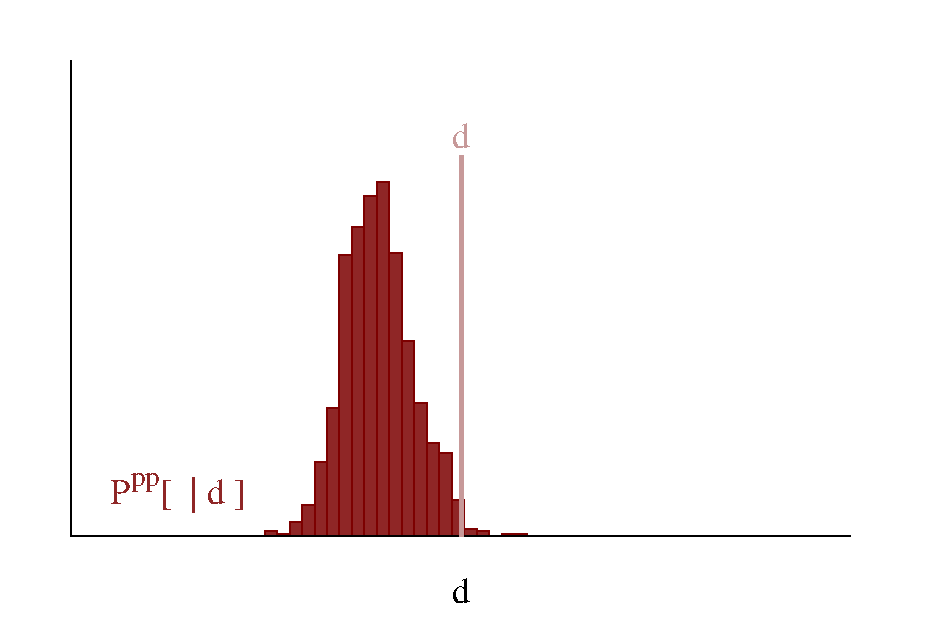
\includegraphics[width=2.75in]{predictive_misfit1.eps} }
\subfigure[]{ 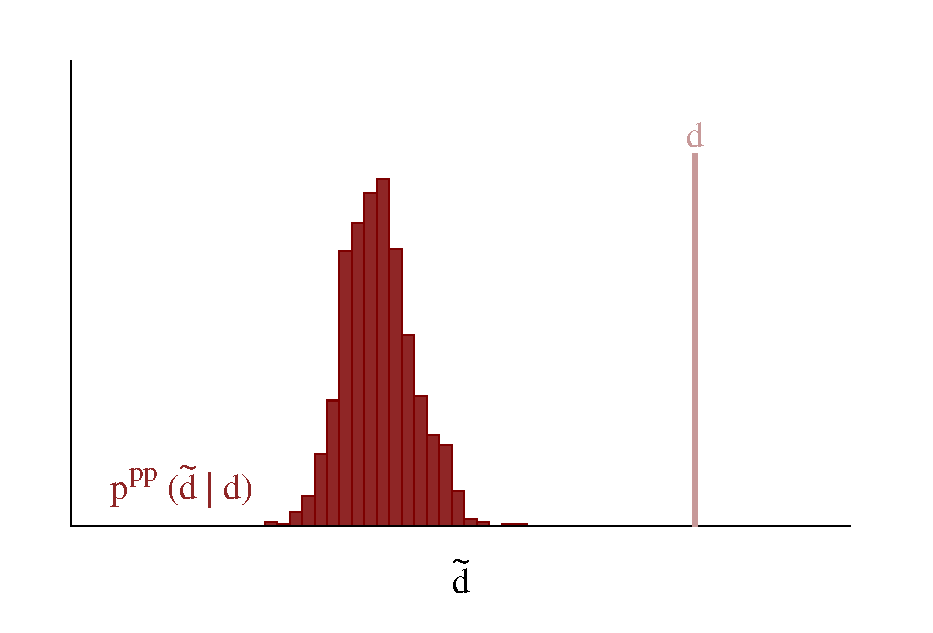
\includegraphics[width=2.75in]{predictive_misfit2.eps} }
\caption{(a) When the measurement, $d$, is consistent with the 
posterior predictive distribution we have no reason to doubt our 
model assumptions, but (b) tension between the measurement and
the posterior predictive distribution indicates that there may be a
problem.  Either the measurement was exceedingly rare or our
model assumptions are insufficient.
}
\label{fig:predictive_misfit}
\end{figure*}

We can also construct a \emph{jackknife posterior predictive
check} by splitting our measurement into two partitions.  Tension
between the marginalized predictive distribution constructed from
one partition and the second partition indicates either an unlikely
measurement or the overfit of the underlying model (Figure
 \ref{fig:predictive_overfit}).

\begin{figure*}
\centering
\subfigure[]{ 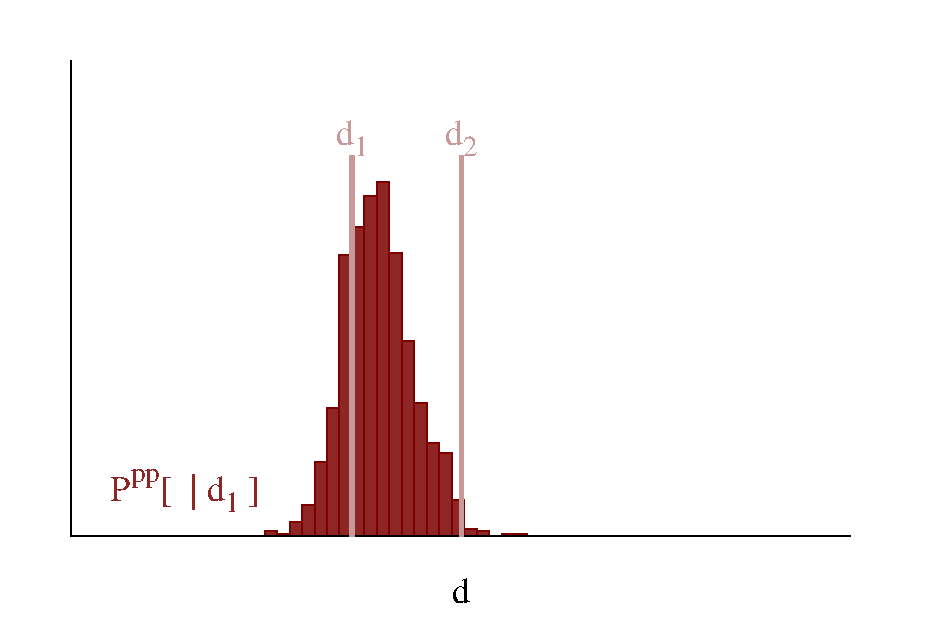
\includegraphics[width=2.75in]{predictive_overfit1.eps} }
\subfigure[]{ 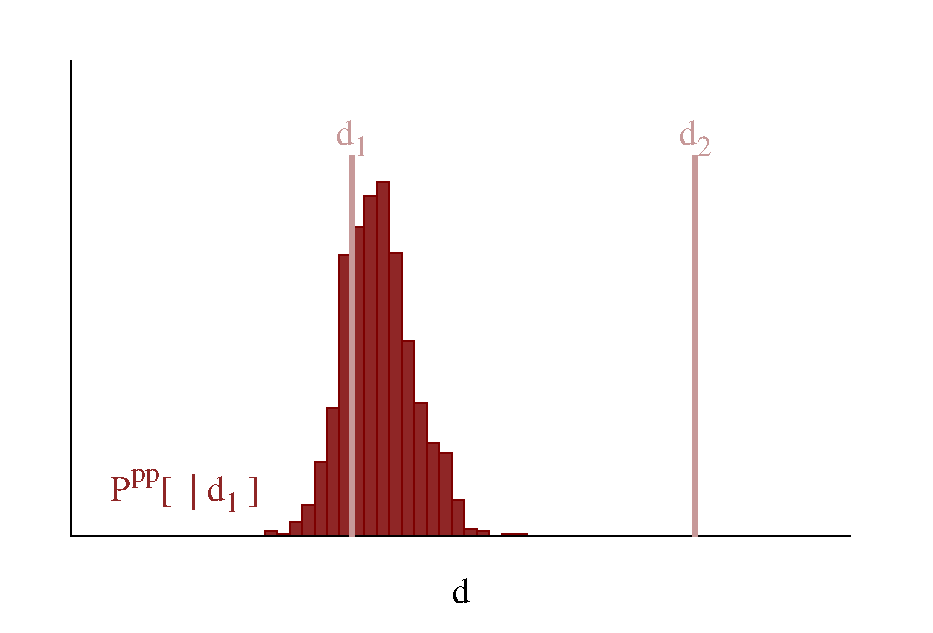
\includegraphics[width=2.75in]{predictive_overfit2.eps} }
\caption{To test for potential overfit we need multiple measurements,
and given only a single measurement this can emulated by splitting
the measurement into two partitions, $d_{1}$ and $d_{2}$.  (a) When 
both measurements are consistent with the posterior predictive 
distribution we have no reason to doubt our model assumptions, but 
(b) tension between the held-out measurement, $d_{2}$ and the 
posterior predictive distribution indicates that the model might be
overfitting to $d_{1}$.  Either the partition generated an exceedingly 
rare measurement or our model assumptions are insufficient.
}
\label{fig:predictive_overfit}
\end{figure*}

As in the general case, these visual predictive checks are not
calibrated and so we cannot discriminate between rare measurements 
and the illegitimacy of our model assumptions.  In practice, however, we 
can appeal to some implicit baseline predictive performance to make 
qualitative judgements as to when the tension is strong enough to be 
suspect.  Suspicion then motivates a careful study of the model 
assumptions that manifest in the chosen component of the 
measurement, and potentially the updating of our model into one more
capable of capturing the intricacies of our data 
(Figure \ref{fig:model_updating}).

\begin{figure*}
\centering
%
\subfigure[]{
\begin{tikzpicture}[scale=0.225, thick]
  \draw[color=white] (-15, 0) -- (15, 0);

  \fill[mid] (0, 0) ellipse (13 and 7);
  \node at (12, -6) {$\mathcal{P}_{D}$};
  
  \draw[color=dark, dashed] (3, -1) ellipse (6 and 3);
  \node[color=white] at (8.5, -3.5) {$\mathcal{S}$};
  
  \fill[color=white] (-7, 3) circle (8pt)
  node[right, color=white] {$\pi_{D}$};
  
  \begin{scope}
    \clip (3, -1) ellipse (6 and 3);
    \foreach \i in {0, 0.05,..., 1} {
      \fill[opacity={exp(-5 * \i*\i)}, dark] (-1.2, 1.2) circle ({2 * \i});      
    }
  \end{scope} 
\end{tikzpicture}
}
%
\subfigure[]{
\begin{tikzpicture}[scale=0.225, thick]
  \draw[color=white] (-15, 0) -- (15, 0);

  \fill[mid] (0, 0) ellipse (13 and 7);
  \node at (12, -6) {$\mathcal{P}_{D}$};
  
  \draw[color=dark, dashed] (1, 0) ellipse (10 and 6);
  \node[color=white] at (8.5, -3.5) {$\mathcal{S}$};
  
   \begin{scope}
    \clip (1, 0) ellipse (10 and 6);
    \foreach \i in {0, 0.05,..., 1} {
      \fill[opacity={exp(-5 * \i*\i)}, dark] (-6, 2) circle ({2 * \i});      
    }
  \end{scope}
  
  \fill[color=white] (-7, 3) circle (8pt)
  node[right, color=white] {$\pi_{D}$};
\end{tikzpicture}
}
\caption{Posterior predictive checks are powerful ways to
make qualitative judgements about the validity of our
model assumptions.  For example, if (a) they suggest 
that our model is misfitting the data then (b) we can
update our model to better capture the features of the
data that are being misfit.
}
\label{fig:model_updating}
\end{figure*}

\section{Bayesian Inference in Practice}

Ultimately, implementing Bayesian inference in practice is
surprisingly straightforward.  Using our expertise about a
system we construct a prior that quantifies our initial
assumptions about the system and a likelihood that
quantifies our assumptions about the latent data generating
process itself.  These two distributions then immediately
define a posterior distribution quantifying our updated uncertainty
about our system, and all inferential summaries and decisions 
reduce to posterior expectations.  Although conceptually simple,
neither of these steps is particularly easy.

Building robust models is an immensely challenging task
that requires both expertise with a given system and familiarity
with the wealth of potential techniques for constructions priors
and likelihoods.  Many of these techniques are discussed in
the Stan manual (and potentially here someday, too), but here
we'd like to highlight a particularly powerful approach to building
likelihoods: \emph{generative modeling}.  

Generative modeling builds up a likelihood from latent parameters
to the measurement sequentially, as if we were trying to simulate
the data generating process itself.  By considering the forward
model we can naturally incorporate causal structure, such as a 
physical model, measurement variation, and systematic effects,
such as bias and measurement error.  At each stage we model
deterministic or stochastic relationships with conditional probability
distributions until we have constructed the complete likelihood.
The generative nature of these models facilities communication
and helps to identify which features may be most suspect, 
motivating targeted posterior predictive checks and model updates.

Once we have specified our assumptions and collected our
data, there many options for approximating the resulting
posterior expectations in practice.  We have discussed many
of these here, and there are always more being developed.
Whichever method we end up using, however, we have to
be careful to validate the accuracy of the estimation, lest a 
biased or highly variable estimator spoil the carefully crafted
model.  Such validation is easier in some computational
techniques than others, and sometimes the fastest algorithms
are the most vulnerable to bias!

Although the modeling and computation steps should ideally
be completely decoupled, in practice they will always interact.
More complex models strain the approximation algorithms in
our toolbox, exhausting our computational resources or
compromising the accuracy of the estimators and, in either 
case, undermining the robustness of our analysis.  In practice
we often have to iterate, using the success or failure of a
fit to inform the next generation of model.  Provided we do
this deliberately, taking care to validate both the model 
assumptions and the fit themselves, we can use Bayesian 
inference to make powerful statements about the world around 
us.

